%%%%%%%%%%%%%%%%%%%%%%%%%%%%%%%%%%%%%%%%%%%%%%%%%%%%%%%%%%%%%%%%%
% Qualificacao de Doutorado / Dept Fisica, CFM, UFSC            %
% Eduardo@UFSC - 2015                                           %
%%%%%%%%%%%%%%%%%%%%%%%%%%%%%%%%%%%%%%%%%%%%%%%%%%%%%%%%%%%%%%%%%

%:::::::::::::::::::::::::::::::::::::::::::::::::::::::::::::::%
%                                                               %
%                          Capítulo 2                           %
%                                                               %
%:::::::::::::::::::::::::::::::::::::::::::::::::::::::::::::::%

%***************************************************************%
%                                                               %
%                        EmLinesDataCube                        %
%                                                               %
%***************************************************************%

\chapter{Linhas de emissão}
\label{sec:emlines}

Os espectros observados carregam uma mistura de energia provenientes de diversas partes distintas
das galáxias (estrelas, gás, poeira, etc). Com a síntese de populações estelares obtêm-se os
espectros relacionados a energia proveniente das estrelas de diferentes idades e composições
químicas, além da correção pela aplicação de alguma lei de extinção por poeira. Subtraindo os
espectros observados dos espectros modelados obtêm-se os espectros residuais, compostos pelas linhas
de emissão. Essas linhas são geradas através de alguns processos físicos, mas basicamente é
resultantes das populações e despopulações dos níveis energéticos dos elementos químicos presentes
no gás.

\section{EmLinesDataCube}
\label{sec:emline:datacube}

Nosso colaborador e membro do Projeto CALIFA {\em Survey}, Rubén García Benito, desenvolveu um
programa que, utilizando dos espectros residuais, faz a medida das linhas de emissão e erros
envolvidos no processo. Este programa faz parte do projeto e por enquanto não está aberto para
utilização da comunidade científica. Acreditamos que essas medidas serão liberadas para a comunidade
científica assim que o último lançamento público de dados do CALIFA for feito (DR3).

Feitas as medidas dos fluxos integrados das linhas de emissão, temos o arcabouço para calcularmos
algumas propriedades que serão fundamentais em nossa pesquisa. Para isso escrevi um objeto em
\textsc{p}y\textsc{thon} que além de organizar os resultados das medidas dos fluxos das linhas de
emissão (provenientes do programa do Rubén) também já calcula metalicidade nebular, extinção por
decremento de Balmer, larguras equivalentes das linhas, assim como os erros propagados em cada
cálculo, etc. Esse objeto foi adicionado ao \pycasso \citep{CidFernandes.etal.2013a} para que os
demais membros do projeto possam utilizá-lo. Nesse objeto encontram-se medidas do fluxo em diversas
linhas de emissão, a posição central da linha, amplitude, desvio padrão, equação para reconstrução
do contínuo em cada linha de emissão, os erros nestas medidas, além das propriedades mencionadas
anteriormente e seus erros propagados.

\subsection{Extinção por decremento de Balmer}
\label{sec:emline:datacube:tauvneb}

Em um modelo que assume que entre o observador e a fonte de energia existe uma
camada difusa, como uma cortina, que extingue a luz diferentemente em cada comprimento de
onda, temos:
\begin{eqnarray}
   F_\lambda^{obs} &=& F_\lambda^{int} e^{-\tau_\lambda} \\
   F_\lambda^{obs} &=& F_\lambda^{int} e^{-(\frac{\tau_\lambda}{\tauV}) \tauV} \\
   \frac{\tau_\lambda}{\tauV} &=& q_\lambda \\
   F_\lambda^{obs} &=& F_\lambda^{int} e^{-q_\lambda \tauV} \\
   \frac{F_\lambda^{obs}}{F_{\lambda^\prime}^{obs}} &=& \
 \frac{F_\lambda^{int} e^{-q_\lambda \tauV}}{F_{\lambda^\prime}^{int} e^{-q_{\lambda^\prime} \tauV}} \\
   \ln \left(\frac{F_\lambda^{obs}}{F_{\lambda^\prime}^{obs}}\right) &=& \
 \tauV (q_{\lambda^\prime} - q_\lambda) \ln \left(\frac{F_\lambda^{int}}{F_{\lambda^\prime}^{int}}\right) \\
   \tauV &=& \frac{1}{(q_{\lambda^\prime} - q_\lambda)} \left[\ln \ 
 \left(\frac{F_\lambda^{obs}}{F_{\lambda^\prime}^{obs}}\right) - \
 \ln \left(\frac{F_\lambda^{int}}{F_{\lambda^\prime}^{int}}\right)\right] 
\end{eqnarray}

\noindent onde $F_\lambda$ é o fluxo em cada comprimento de onda, $\tau_\lambda$ é o coeficiente de
profundidade óptica para o comprimento de onda $\lambda$ e $\tauV$ é o coeficiente de profundidade
óptica na banda V.

A poeira existente ao redor das regiões de formação estelar é criada principalmente pelo própria
formação estelar. Assumindo um modelo de extinção \citet[neste trabalho assumimos][]{CCM1989a},
podemos calcular qual o coeficiente de extinção para essas regiões nebulares utilizando o fato de
que apesar do avermelhamento o espectro observado, a razão entre os fluxos intrínsecos das linhas de
\Halpha e de \Hbeta varia um pouco com a metalicidade, de uma forma muito suave, assim assumimos
constante e igual a $2,86$. Com isso temos:
\begin{equation}
	\tauVN = \frac{1}{(q_{\Hbeta} - q_{\Halpha})} \ln \left( \frac{F_{\Halpha}^{obs}/F_{\Hbeta}^{obs}}{2,86} \right).
\end{equation}
\noindent Nessa equação, os $q_\lambda$ são provenientes do modelo adotado. O erro propagado para
$\tauVN$ é:
\begin{eqnarray}
	\tauVN &\equiv& \tauVN(F_{\Halpha}^{obs}, F_{\Hbeta}^{obs}) \\
	\epsilon (\tauVN) &=& \sqrt{\left(\del{\tauVN}{F_{\Halpha}^{obs}}\right)^2 \
\epsilon (F_{\Halpha}^{obs})^2 + \left(\del{\tauVN}{F_{\Hbeta}^{obs}}\right)^2 \
\epsilon (F_{\Hbeta}^{obs})^2 } \\
	\del{\tauVN}{F_{\Halpha}^{obs}} &=& \frac{1}{F_{\Halpha}^{obs} (q_{\Hbeta} - q_{\Halpha})} \\
	\del{\tauVN}{F_{\Hbeta}^{obs}} &=& - \frac{1}{F_{\Hbeta}^{obs} (q_{\Hbeta} - q_{\Halpha})} \\
	\epsilon (\tauVN) &=& \frac{1}{(q_{\Hbeta} - q_{\Halpha})} \
\sqrt{\left(\frac{\epsilon (F_{\Halpha}^{obs})}{F_{\Halpha}^{obs}}\right)^2 + \
\left(\frac{\epsilon (F_{\Hbeta}^{obs})}{F_{\Hbeta}^{obs}}\right)^2 }
\end{eqnarray}

\subsection{Metalicidade Nebular}
\label{sec:emline:datacube:Zneb}

Os indicadores de metalicidade nebular mais utilizados são aqueles que se baseiam na abundância de
oxigênio no gás ($\log$ (O3N2) e N2). As calibrações destes dois indicadores utilizadas pelo nosso
projeto foram feitas por \citet{Marino.etal.2013a} de forma empírica utilizando medidas de
temperatura eletrônica de 603 regiões \Hii e mais medidas nebulares de 3423 regiões \Hii mapeadas
por \citet{Sanchez.etal.2013a}. O valor encontrado pelos autores foi:
\begin{equation}
	12 + \log \textrm{(O/H)} = 8.533[\pm0.012] - 0.214[\pm0.012]\times \textrm{O3N2}
\end{equation}
\noindent conforme pode ser vista na Fig. \ref{fig:Marino2013_O3N2}.

\begin{figure}
	\centering
	%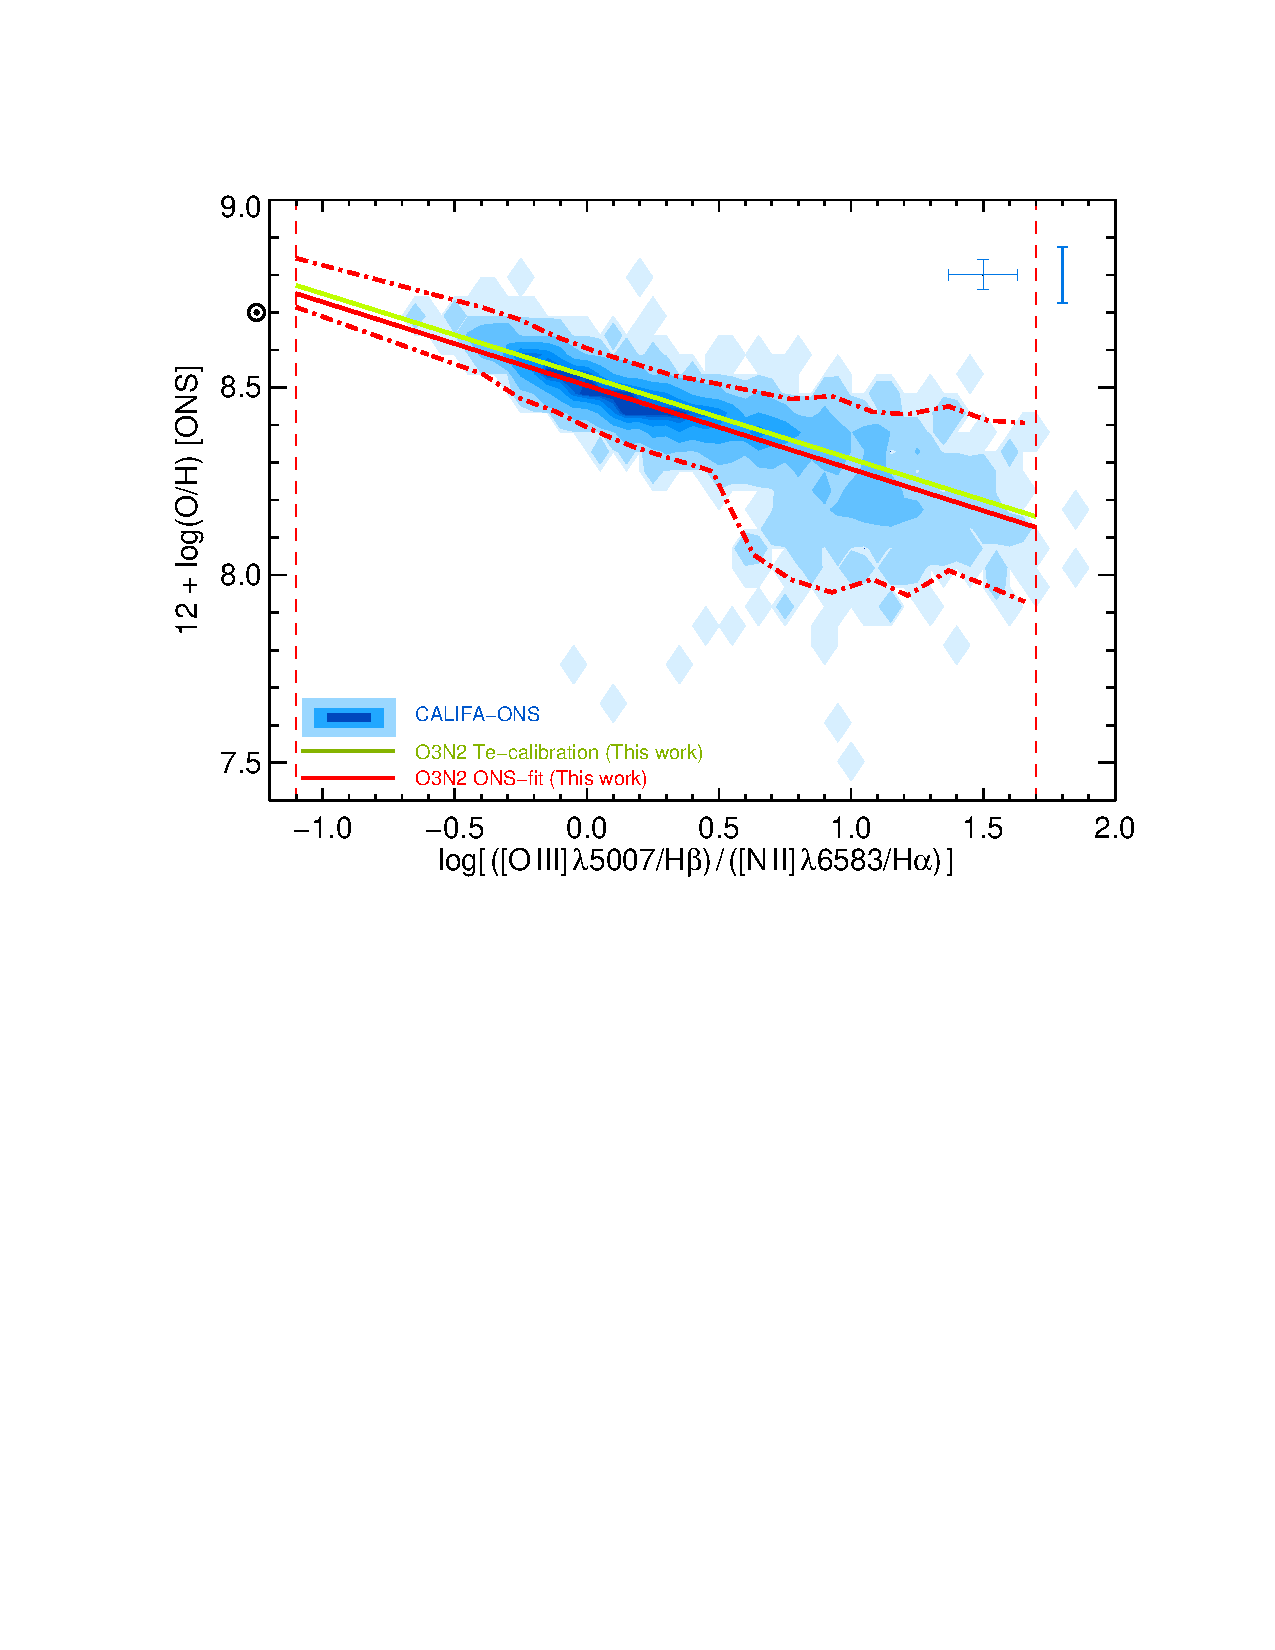
\includegraphics[width=0.3\columnwidth]{figuras/O3N2_CALIFA.pdf}
	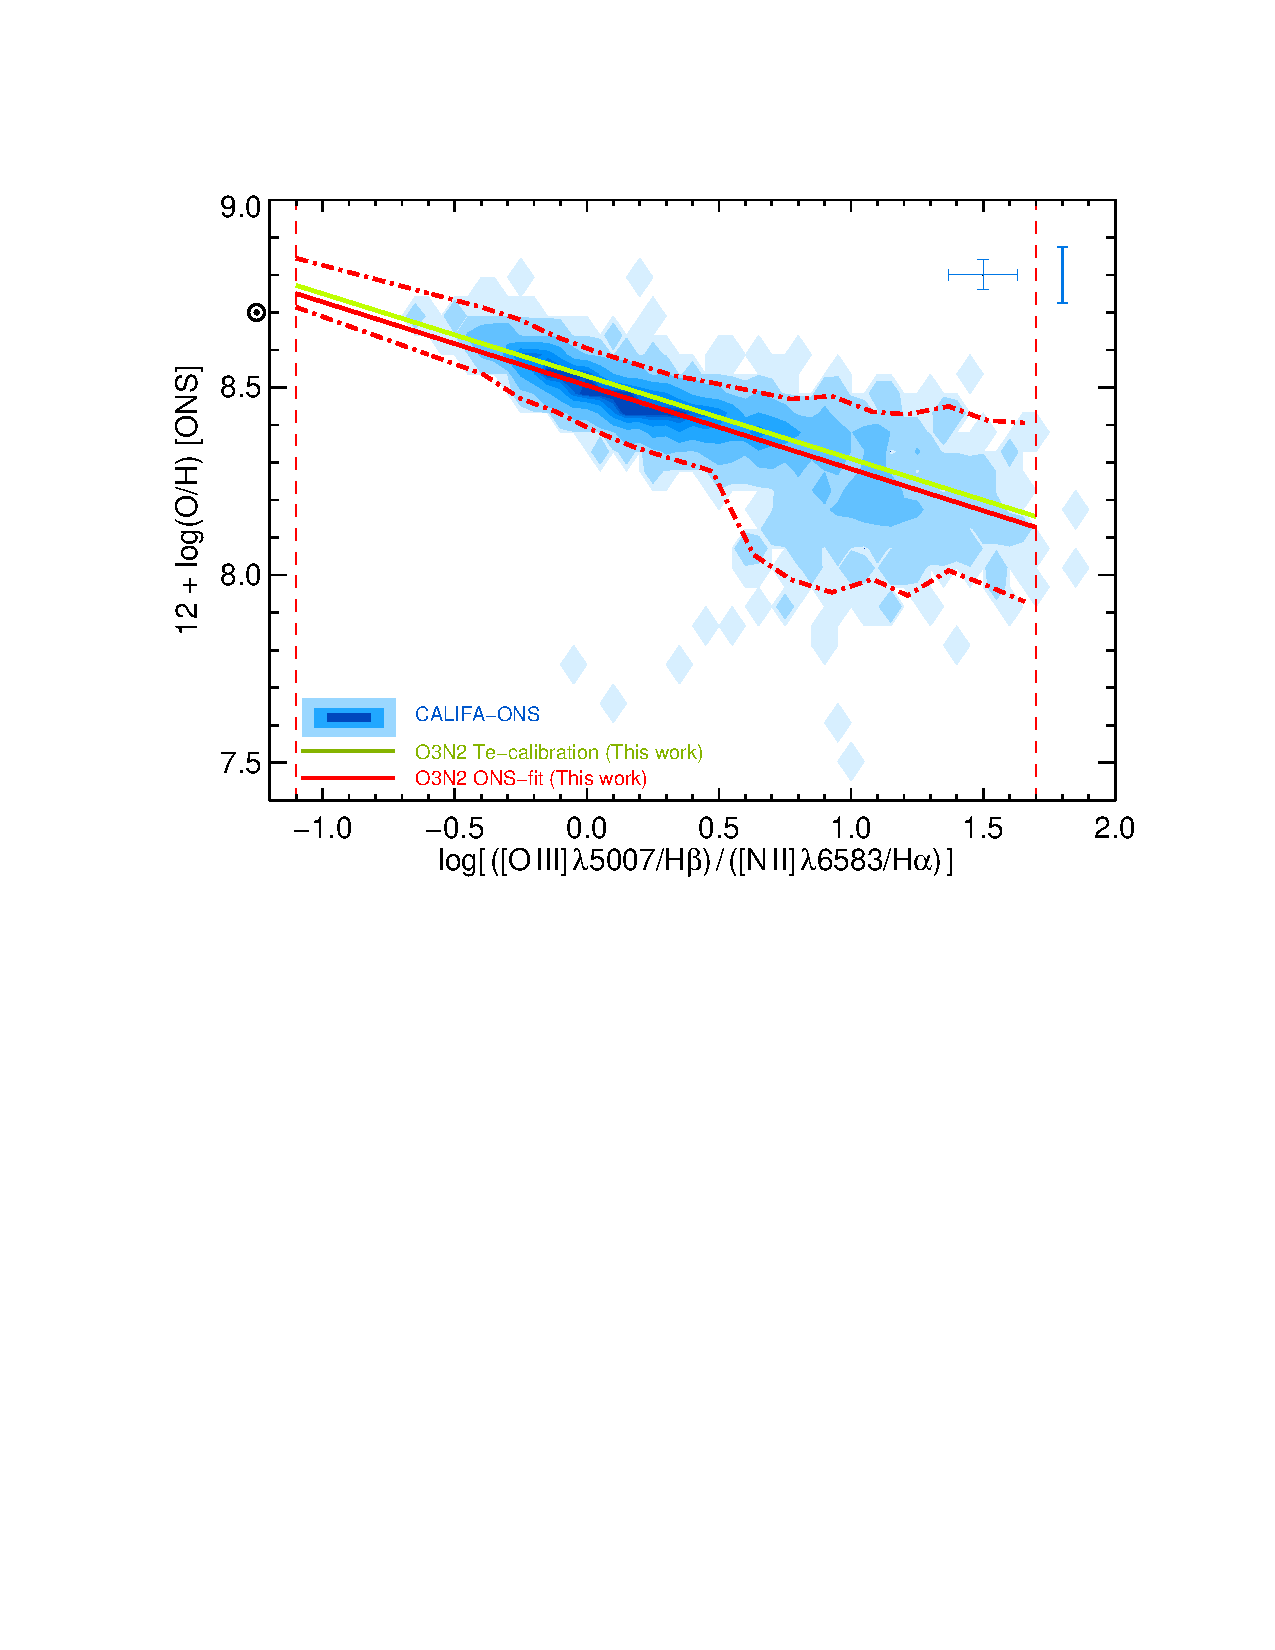
\includegraphics[scale=0.8, trim=2cm 13cm 2cm 3cm, clip]{figuras/O3N2_CALIFA.pdf}
	\caption[Calibração da abundância de oxigênio no gás]{Calibração da abundância de oxigênio 
	nebular	para 3423 regiões \Hii mapeadas por \citet{Sanchez.etal.2013a}. Figura retirada de 
	\citet{Marino.etal.2013a}}
	\label{fig:Marino2013_O3N2}
\end{figure}

\subsection{Exemplo de utilização}
\label{sec:emline:datacube:exemple}

Com a criação do objeto {\sc EmLinesDataCube} e adição ao \pycasso torna o processo de
análise e produção de gráficos extremamente simples. Vamos a um exemplo de como produzir um gráfico
BPT \citep{Baldwin.Phillips.Terlevich.1981a} que utiliza fluxos de quatro linhas de emissão
($\Halpha$, $\Hbeta$, $\OIII$ e $\NII$).

\begin{figure}
	\begin{python}
import numpy as np
from matplotlib import pyplot as plt
from pycasso import fitsQ3DataCube

CALIFASuperFits='K0277.fits'
EmLinesFits='K0277.EML.fits'

# Carregando arquivos FITS
K = fitsQ3DataCube(CALIFASuperFits)
K.loadEmLinesDataCube(EmLinesFits)
# Agora todos as informacoes sobre as linhas de 
# emissao estao instanciadas em K.EL

# Indices dos vetores aonde estao armazenados os 
# fluxos de cada linha
i_Ha = K.EL.lines.index('6563')
i_Hb = K.EL.lines.index('4861')
i_O3 = K.EL.lines.index('5007')
i_N2 = K.EL.lines.index('6583')
Ha_obs__z = K.EL.flux[i_Ha, :]
Hb_obs__z = K.EL.flux[i_Hb, :]
N2_obs__z = K.EL.flux[i_N2, :]
O3_obs__z = K.EL.flux[i_O3, :]

# Razao entre os fluxos de N2/Ha e O3/Hb
N2Ha__z = np.log10(N2_obs__z) - np.log10(Ha_obs__z)
O3Hb__z = np.log10(O3_obs__z) - np.log10(Hb_obs__z)

# Grafico 
f = plt.figure()
ax = f.gca()
ax.scatter(N2Ha__z, O3Hb__z, color = 'black')
ax.set_xlabel(r'$\log\ [NII]/H\alpha$')
ax.set_ylabel(r'$\log\ [OIII]/H\beta$')
f.savefig('%s-BPT.png' % K.califaID)
	\end{python}
	\caption[Exemplo de programa utilizando o EmLinesDataCube.]
	{Exemplo de programa utilizando os fluxos de \Halpha, \Hbeta, \OIII e \NII 
	para construção de um gráfico BPT.}
	\label{fig:BPTprog}
\end{figure}
 
% End of this chapter
